% 對我來說太複雜。

\section{pgfplots}
%% ------------------------------------------------------------
\begin{tikzpicture}
   \begin{loglogaxis}[
        title =Convergence Plot,
        xlabel={Degrees of freedom},
        ylabel={$L 2$ Error},
        grid=major,
        legend entries ={$d=2$,$d=3$,$d=4$},
    ]
        \addplot table {data d2.dat};
        \addplot table {data d3.dat};
        \addplot table {data d4.dat};
        \addplot table[
            x=dof,
            y={create col/linear regression ={y=l2 err,
            variance list ={1000,800,600,500,400,200,100}}}
        ] {data d4.dat};
    \end{loglogaxis}
\end{tikzpicture}

%% ------------------------------------------------------------
\begin{tikzpicture}
    \begin{axis}[
        title =Inv. cum. normal,
        xlabel={$x$},
        ylabel={$y$},
        ymin=−3, ymax=3,
        minor y tick num=1,
    ]
        \addplot[blue] table {./invcum.dat};
    \end{axis}
\end{tikzpicture}

%% ------------------------------------------------------------
\begin{tikzpicture}
    \begin{axis}[
        domain=0:10,scaled ticks=false,
        ymax=2000,ymin=2,minor tick num=1,
        xlabel=$x$, ylabel=$f(x)$,
    ]
        \addplot+[no marks,thick] {xˆ3};
        \addlegendentry{$xˆ3$}; 
        \addplot+[no marks,thick] {x∗(2)ˆx};
        \addlegendentry{$2ˆx\,x$};
    \end{axis}
\end{tikzpicture}

%% ------------------------------------------------------------

\begin{tikzpicture}
    \pgfmathdeclarefunction{sincf}{1}{%
        \pgfmathparse{(abs(#1)<0.01) ? 1 : sin(pi∗#1 r)/(pi∗#1)}%
    }
    \begin{axis}
        \addplot {sincf(\x)};
    \end{axis}
\end{tikzpicture}

%% ------------------------------------------------------------
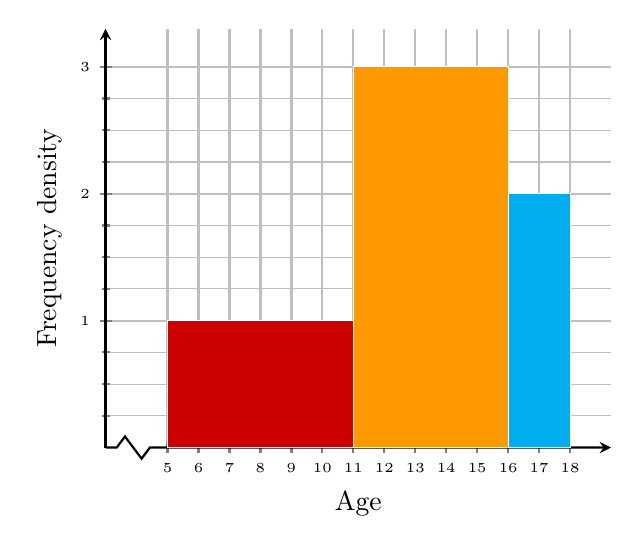
\begin{tikzpicture}
    \begin{axis}[width=8cm,
        axis lines =center,
        xmin=3,xmax=19,
        ymin=0,ymax=3,
        grid=major,
        yminorgrids,
        ylabel near ticks ,
        xlabel near ticks ,
        major grid style ={thick},
        tick style ={thick},
        axis line style ={thick},
        xlabel=Age,
        ylabel=Frequency density,
        xtickmin=4,
        xtick ={5,6,...,18},
        ytick={0,1,2,3},
        minor y tick num=3,
        axis x discontinuity =crunch,
        ticklabel style ={font=\tiny},
        enlarge x limits ={upper,value=0.02},
        enlarge y limits ={upper,value=0.1}
    ]
    \addplot[ybar interval , fill =red!80!black,draw=white]
        coordinates {(5,1)(11,3)};
    \addplot[ybar interval , fill =orange!80!yellow,draw=white]
        coordinates {(11,3)(16,2)};
    \addplot[ybar interval , fill =cyan,draw=white]
        coordinates {(16,2)(18,2)};
    \end{axis}
\end{tikzpicture}

source: \url{http://konoyonohana.blog.fc2.com/blog-entry-140.html}